\documentclass[a4paper,11pt]{article}

\usepackage[utf8]{inputenc}
\usepackage[T1]{fontenc}
\usepackage[ngerman]{babel}
\usepackage{graphicx}
\usepackage{array}
\usepackage{booktabs}
\usepackage{longtable}
\usepackage{tabularx}
\usepackage{makecell}
\renewcommand\theadfont{\bfseries\small}
\usepackage{amsmath}
\usepackage{float}

\usepackage[scaled]{helvet}
\renewcommand{\familydefault}{\sfdefault}

\usepackage[a4paper, top=2cm, bottom=2cm, left=2cm, right=2cm]{geometry}

\usepackage{setspace}
\setstretch{1.5}

\setlength{\parindent}{0pt}
\setlength{\parskip}{6pt}

\usepackage{microtype}
\sloppy
\hyphenpenalty=1000
\tolerance=3000

\renewcommand{\footnotesize}{\fontsize{10}{12}\selectfont}

\setcounter{secnumdepth}{3}
\setcounter{tocdepth}{3}

\usepackage{titlesec}
\titleformat{\section}{\normalfont\fontsize{12}{14}\bfseries}{\thesection}{1em}{}
\titleformat{\subsection}{\normalfont\fontsize{12}{14}\bfseries}{\thesubsection}{1em}{}
\titleformat{\subsubsection}{\normalfont\fontsize{12}{14}\bfseries}{\thesubsubsection}{1em}{}

\usepackage[
  colorlinks=true,
  linkcolor=black,
  citecolor=blue,
  filecolor=black,
  urlcolor=blue
]{hyperref}
\usepackage[capitalise,nameinlink]{cleveref}

\usepackage{fancyhdr}
\pagestyle{fancy}
\fancyhf{}
\renewcommand{\headrulewidth}{0pt}
\fancyfoot[C]{\thepage}

\usepackage[german=quotes]{csquotes}

\usepackage[backend=biber, style=apa]{biblatex}
\addbibresource{references.bib}

\usepackage{titling}

\usepackage{listings}
\usepackage{xcolor}
\lstset{
    basicstyle=\ttfamily\small,
    breaklines=true,
    frame=single,
    numbers=left,
    numberstyle=\tiny\color{gray},
    keywordstyle=\color{blue},
    commentstyle=\color{green!50!black},
    stringstyle=\color{red!60!black},
    showstringspaces=false,
    tabsize=4
}

\begin{document}

\begin{titlepage}
    \thispagestyle{empty}
    \centering
    \vspace*{5cm}
    {\Huge\bfseries Projekt: Data Analysis DLBDSEDA02\_D \par}
    \vspace{1cm}
    {\Large Portfolioteil 2 -- Erarbeitungs-/Reflexionsphase \par}
    \vspace{0.3cm}
    {\large Aufgabe 1: NLP-Techniken anwenden, um eine Textsammlung zu analysieren \par}
    \vspace{0.5cm}
    {\large Studiengang: Angewandte Künstliche Intelligenz \par}
    \vspace{0.5cm}
    {\large Sven Behrens \par}
    \vspace{0.5cm}
    {\large Matrikelnummer: 42303511 \par}
    \vspace{0.5cm}
    {\large \today \par}
    \vspace{0.5cm}
    {\large Tutor: Prof.~Dr.~Frank Passing \par}
\end{titlepage}

\pagenumbering{arabic}
\setcounter{page}{1}

% ============================================================
% ERLÄUTERUNG DER IMPLEMENTIERUNG
% ============================================================
\section{Erläuterung der Implementierung}

Der vollständige, versionskontrollierte Quellcode ist im GitHub-Repository verfügbar:
\url{https://github.com/svenb23/DataAnalysis}

Die Implementierung erfolgte in einer virtuellen Python-Umgebung (venv), deren Abhängigkeiten
über eine \texttt{requirements.txt} reproduzierbar installiert werden können. Der Workflow ist
in fünf modulare Skripte gegliedert, die sequentiell ausgeführt werden:

Im ersten Schritt (\texttt{01\_load\_data.py}) wurde die CFPB Consumer Complaint Database \parencite{cfpb2024} geladen
und auf Einträge mit vorhandenem Freitext gefiltert. Aus den ca.~3,7~Millionen relevanten
Beschwerden wurde ein zufälliges Sample von 50.000~Einträgen gezogen.

Die Vorverarbeitung (\texttt{02\_preprocessing.py}) umfasste Lowercasing, Entfernung von
Sonderzeichen, URLs und CFPB-Redaktionen sowie Tokenisierung, Stoppwort-Entfernung und
Lemmatisierung mittels spaCy.

Für die Vektorisierung (\texttt{03\_vectorization.py}) wurden TF-IDF (5.000~Features) und
Word2Vec (100-dimensionale Vektoren) eingesetzt. TF-IDF erwies sich als geeigneterer Input
für die nachfolgende Themenextraktion, da Word2Vec eine Aggregation auf Dokumentebene erfordert.

Die Themenextraktion (\texttt{04\_topic\_modeling.py}) erfolgte mit LDA und NMF (jeweils 10~Topics).
NMF lieferte schärfer abgegrenzte und besser interpretierbare Themen (siehe \cref{fig:topwords} im Anhang),
während LDA stärkere Überlappungen zwischen Topics zeigte. Die extrahierten Themen (z.\,B. Debt Collection,
Identity Theft, Mortgage) stimmen mit den Produktkategorien der Metadaten überein
(siehe \cref{fig:products} im Anhang), was die Validität der Ergebnisse stützt.

Abschließend wurden die Ergebnisse als Wortwolken (\cref{fig:wordclouds}), Balkendiagramme der Top-Wörter pro Topic und
Verteilung der Dokumente über die Topics (\cref{fig:topicdist}) visualisiert (\texttt{05\_visualization.py}).

\newpage
\printbibliography[title=Literaturverzeichnis]

\newpage
\appendix
\section*{Anhang}
\addcontentsline{toc}{section}{Anhang}

\begin{figure}[H]
\centering
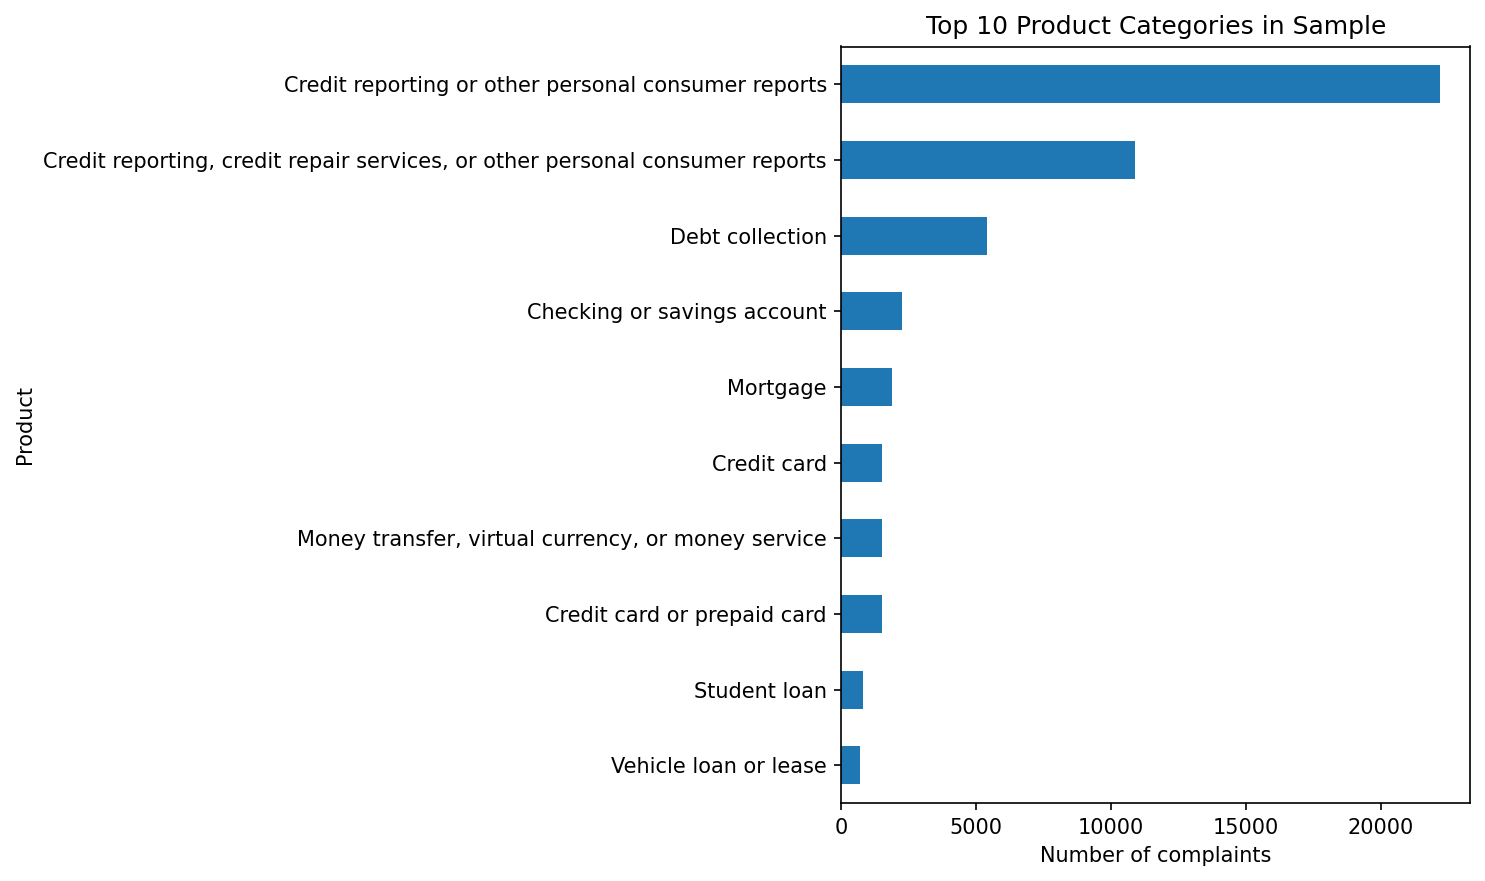
\includegraphics[width=\textwidth]{../results/product_distribution.png}
\caption{Verteilung der Produktkategorien im Sample (Top 10)}
\label{fig:products}
\end{figure}

\begin{figure}[H]
\centering
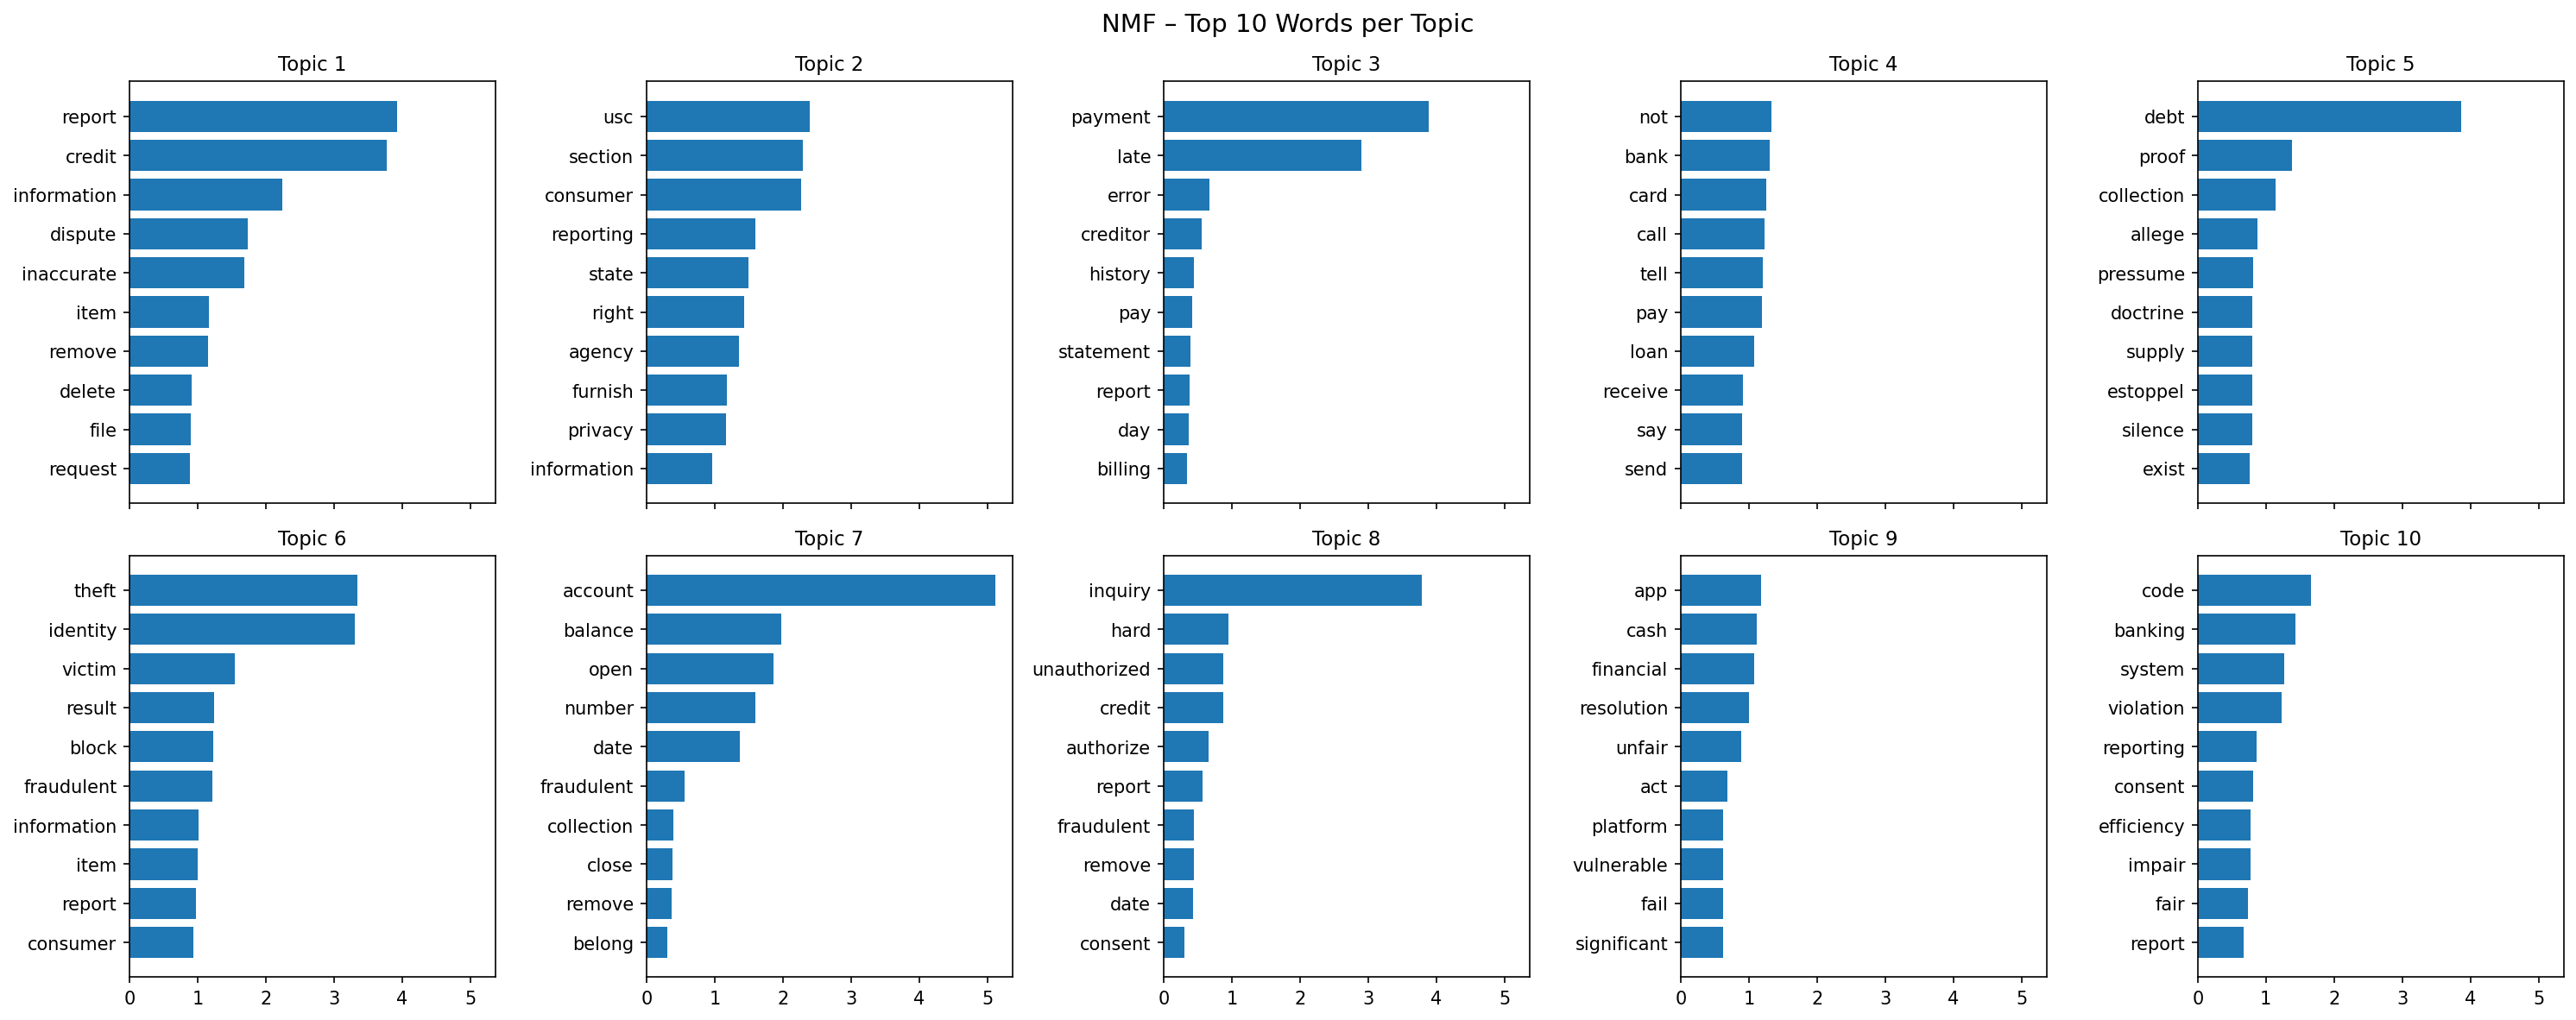
\includegraphics[width=\textwidth]{../results/nmf_top_words.png}
\caption{NMF -- Top 10 Wörter pro Topic}
\label{fig:topwords}
\end{figure}

\begin{figure}[H]
\centering
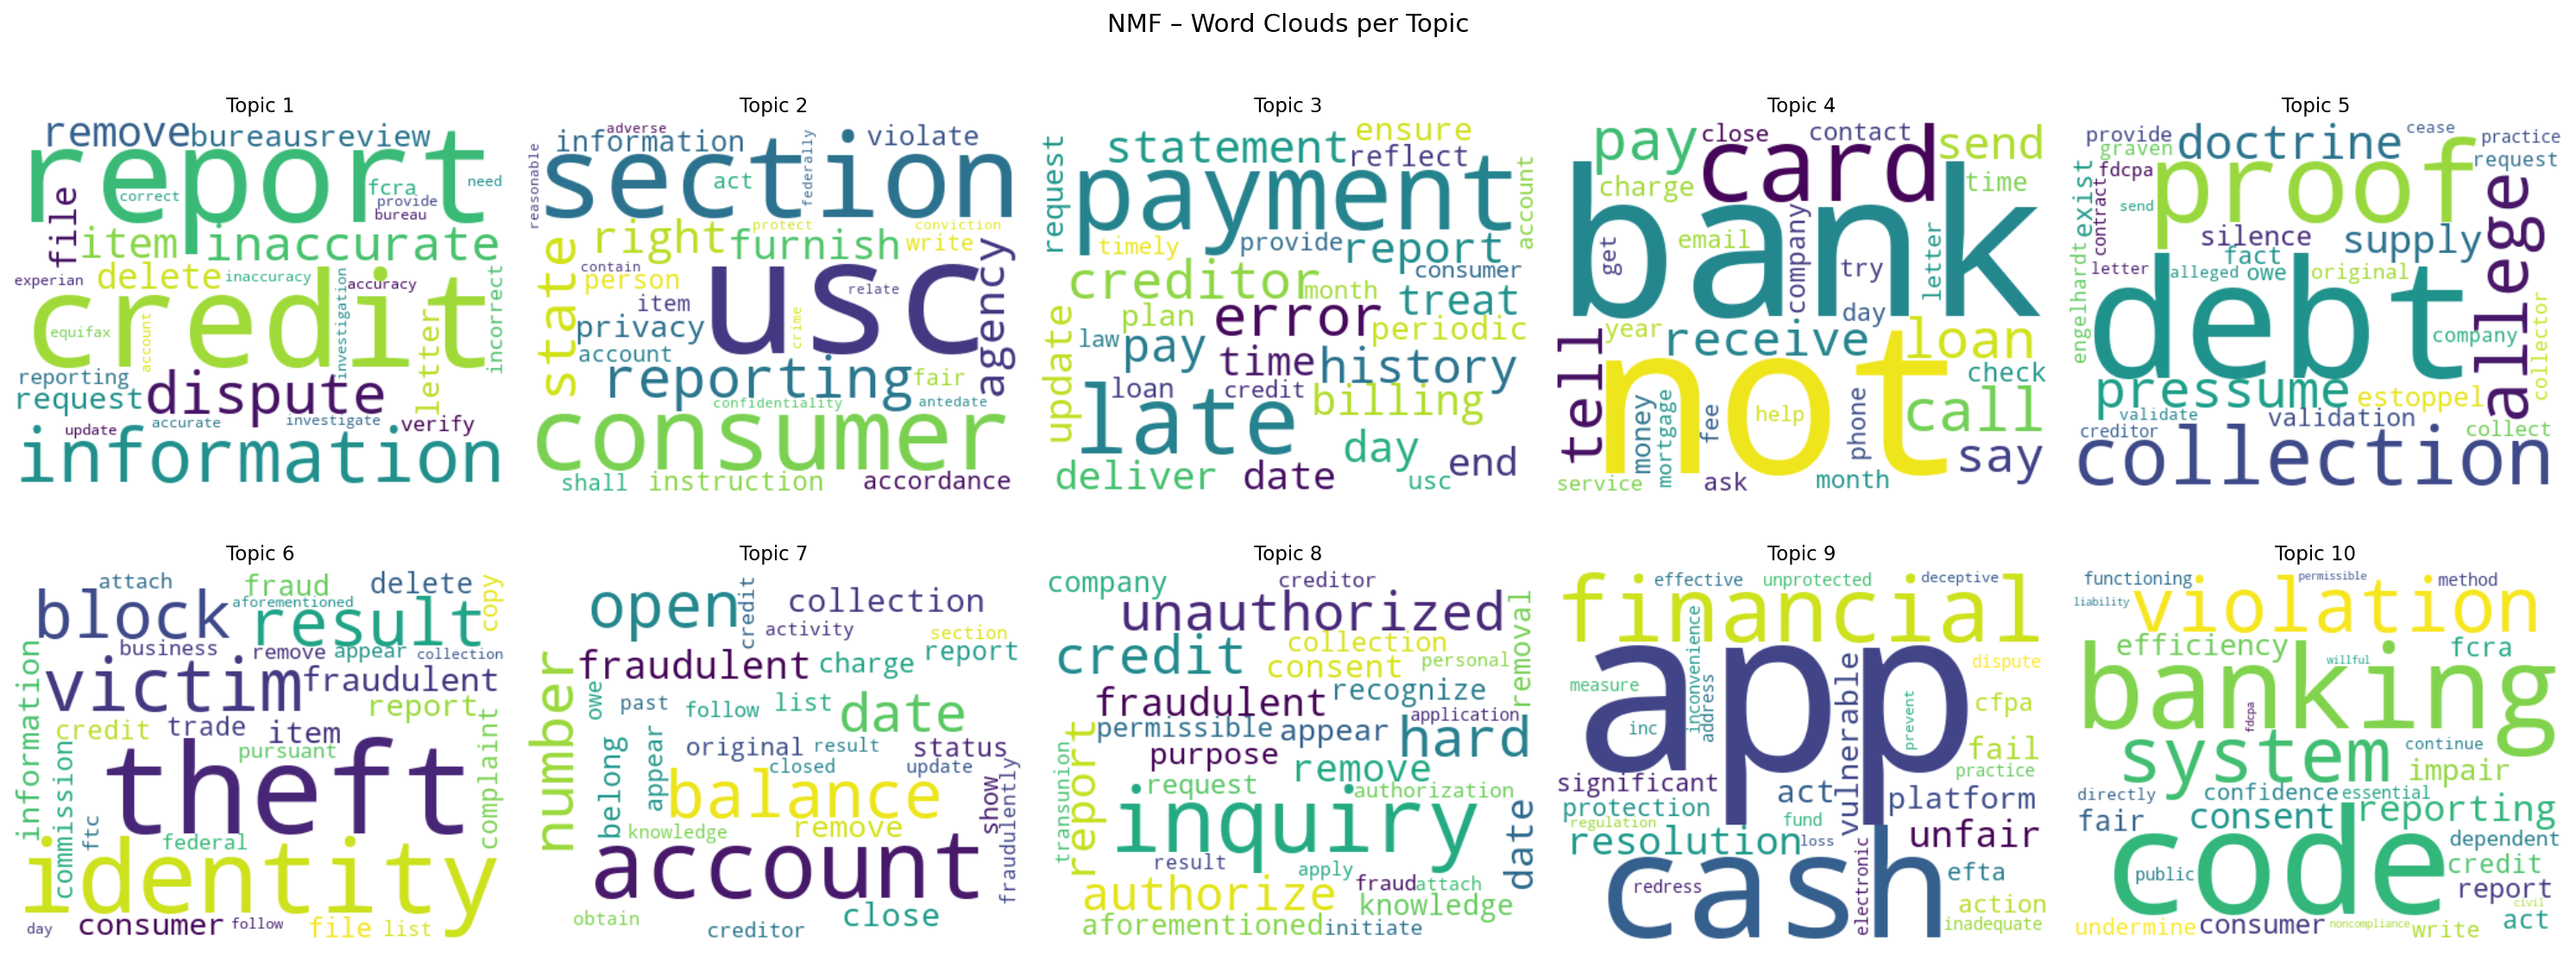
\includegraphics[width=\textwidth]{../results/nmf_wordclouds.png}
\caption{NMF -- Wortwolken pro Topic}
\label{fig:wordclouds}
\end{figure}

\begin{figure}[H]
\centering
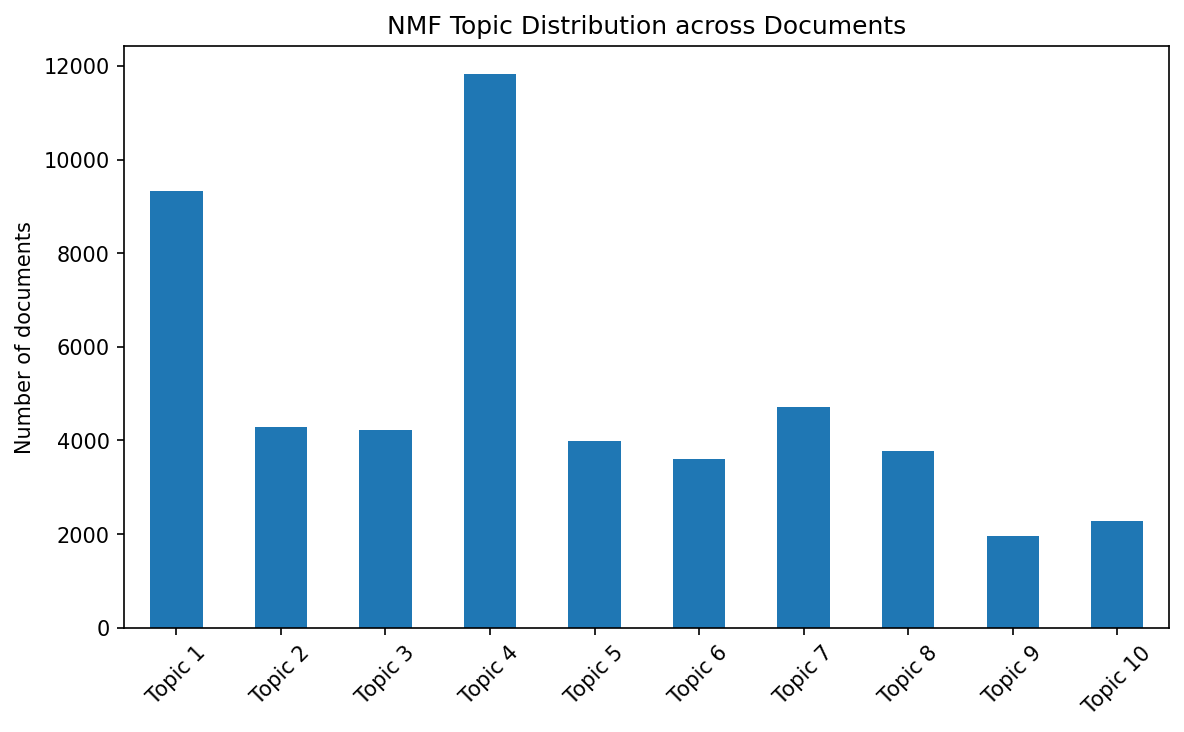
\includegraphics[width=0.8\textwidth]{../results/nmf_topic_distribution.png}
\caption{NMF -- Verteilung der Dokumente über die Topics}
\label{fig:topicdist}
\end{figure}

\end{document}
